\documentclass[a4paper,french]{paper}
\usepackage{../../_latex_assets/villemejane_iogs_ceti}

%Informations about this document 
%------------------------------------------
\def\module{Ingénierie Electronique pour le Traitement de l'Information}
\def\moduleAbrege{6N-047-SCI / IéTI}
\def\annee{}

\def\titre{TD 2 / Pilotage d'une source à diodes}
\author{Julien VILLEMEJANE}

\subtitle{TD 2}
\institution{LEnsE / Institut d'Optique Graduate School}

\title{\titre}
\begin{document} 
%Beginning First Page. 
%------------------------------------------
\enteteThematiqueObligatoire{}

%Beginning Content. 
%------------------------------------------
\vspace{-1cm}
%%%%%%%%%%%%%%%%%%%
\subsection*{Transistors bipolaires}

Les transistors bipolaires sont des composants amplificateurs de courant à 3 broches : l'émetteur, le collecteur et la base.

\begin{center}
	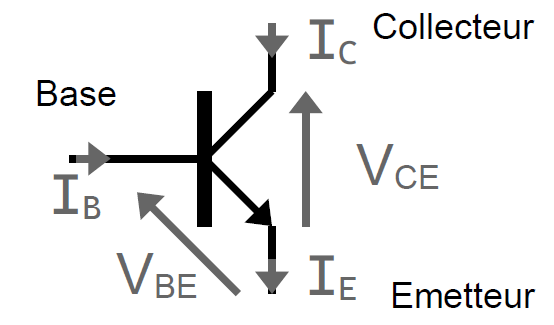
\includegraphics[width=5cm]{images/bipolaire.png}
\end{center}

Les différents courants et tensions sont régis par les relations suivantes :

$$I_C = \beta \cdot I_B \qquad et \qquad I_E = I_C + I_B$$

$$I_C = \beta \cdot I_{BS} \cdot \exp(V_{BE}/U_T)$$

où $U_T$, $I_{BS}$ et $\beta$ sont des paramètres intrinsèques du transistor.


%%%%%%%%%%%%%%%%%%%

\encadreTDExo{1 - Miroir de courant}{
On s'intéresse au montage suivant :

\begin{center}
	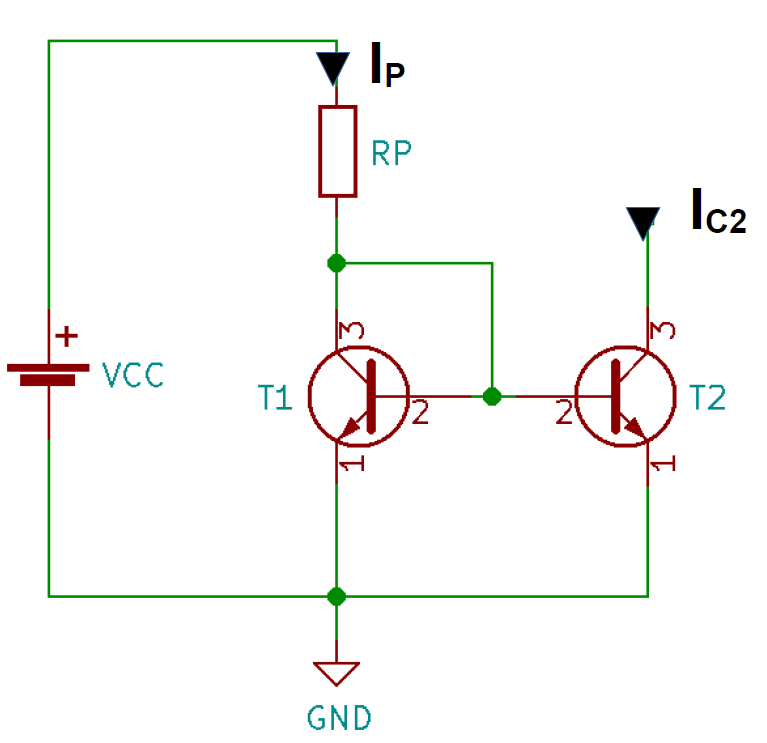
\includegraphics[width=7cm]{images/mirroir_courant_1.png}
\end{center}


\begin{enumerate}
	\item Calculez $I_{C2}$ en fonction de $I_P$.
	\item Calculez la puissance dissipée par la résistance $R_P$
	\item Retrouve-t-on cette structure dans le composant AL5809 (dont une partie de la documentation est fournie en annexe) ?
	\item Expliquez le fonctionnement de ce composant. Quel est l'intérêt du montage de la figure 3 (p.5 de la documentation) par rapport à celui de la figure 2 ?
\end{enumerate}
}

Pour le transistor T1, on notera $I_{C1}$ le courant rentrant dans le collecteur, $I_{B1}$ le courant rentrant dans la base, $I_{E1}$ le courant sortant de l'émetteur et $V_{BE1}$ la tension entre la base et l'émetteur.

Pour le transistor T2, on notera $I_{C2}$ le courant rentrant dans le collecteur, $I_{B2}$ le courant rentrant dans la base, $I_{E2}$ le courant sortant de l'émetteur et $V_{BE2}$ la tension entre la base et l'émetteur.

\medskip

\rule{\linewidth}{.5pt}

\textbf{1 - Calcul de $I_{C2}$}

Par la loi des noeuds, on obtient : 

$I_P =  I_{C1} + I_{B1} + I_{B2}$

Par la loi des mailles, on obtient également que : $V_{BE1} = V_{BE2}$.

Comme les deux transistors sont identiques : $I_{B1} = I_{B2} = I_{B}$.

On sait aussi que $I_{C1} = \beta \cdot I_{B1}$.


\medskip

On obtient alors que :

$$\boxed{I_P =  \beta \cdot I_{B} + 2 \cdot I_{B}}$$

\medskip

On sait que $I_{C2} = \beta \cdot I_{B2}$ 

Ainsi : $$\boxed{I_{C2} =  \frac{\beta}{\beta + 2} \cdot I_{P}}$$


Si $\beta >> 1$, alors l'expression suivante peut se simplifier en $I_{C2} = I_{P}$

\medskip

On peut également calculer $I_P$ à partir des autres éléments.

Par la loi des mailles, on obtient que : $V_{CC} - R_P \cdot I_P + V_{BE1} = 0$

On peut ainsi montrer que le courant $I_P$ est paramétrable par le choix de $R_P$ et $V_{CC}$. 

$$\boxed{I_{P} =  \frac{V_{CC} - V_{BE1}}{R_P}}$$


\medskip

\rule{\linewidth}{.5pt}

\textbf{2 - Puissance dissipée par $R_P$}

La puissance dissipée par $R_P$ vaut : $P_R = R_P \cdot I_P^2$

$$\boxed{P_{R} =  \frac{(V_{CC} - V_{BE1})^2}{R_P}}$$

\rule{\linewidth}{.5pt}

\textbf{3 - Composant AL5809}

A la page 2 de la documentation, on trouve le schéma suivant : 

\begin{center}
	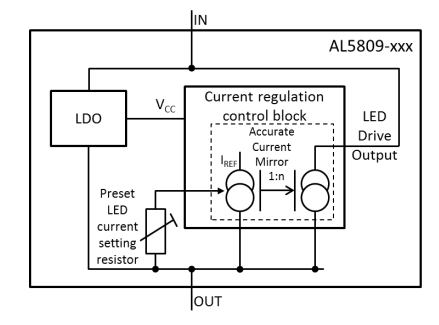
\includegraphics[width=7cm]{images/AL5809_mirroir_courant_p2.png}
\end{center}

On retrouve au centre un miroir de courant (basé sur le principe précédent). La résistance $R_P$ du montage précédent est ici un potentiomètre interne (\textit{Preset LED current setting resistor}). La tension $V_{CC}$ est régulée par un composant LDO (\textit{Low Dropout Regulator}).

\rule{\linewidth}{.5pt}

\textbf{4 - Fonctionnement du composant AL5809}

Le composant final ne possède que 2 broches : la broche IN par lequel le courant va entrer et une broche OUT par lequel le courant va sortir. L'ensemble du montage vu précédemment est intégré et auto-régulé en courant (figure 2).

Il est alors possible de les mettre en parallèle pour obtenir un courant plus important, mais toujours régulé (figure 3).

\newpage
%------------------------------------------
%%%%%%%%%%%%%%%%%%%
\encadreTDExo{2 - Driver de LEDs}{
On donne le schéma interne du composant NCR320U :

\begin{center}
	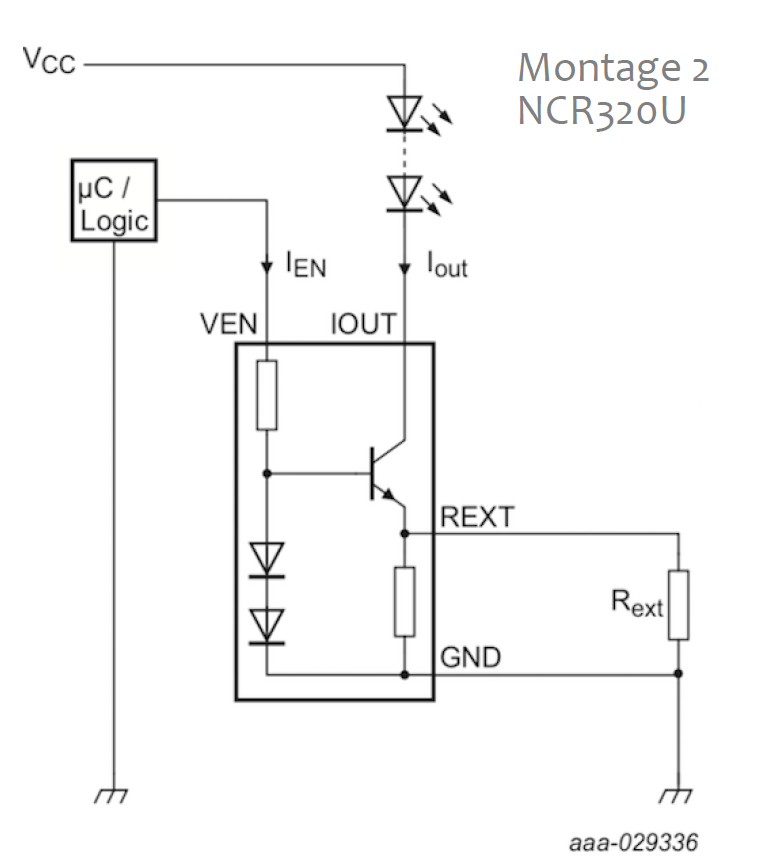
\includegraphics[width=10cm]{images/mirroir_courant_2.png}
\end{center}

\begin{enumerate}
	\item Calculez le courant $I_{out}$ en fonction de $R_{ext}$ et précisez le rôle de cette résistance.
	\item Calculez le courant $I_{en}$ en fonction de $V_{en}$ et précisez le rôle de cette tension.
	\item Expliquez le rôle de ce composant et son fonctionnement.
\end{enumerate}
}

on notera $I_{C}$ le courant rentrant dans le collecteur, $I_{B}$ le courant rentrant dans la base, $I_{E}$ le courant sortant de l'émetteur et $V_{BE}$ la tension entre la base et l'émetteur.

On notera $R_E$ la résistance interne du composant reliée à l'émetteur du transistor.

On notera $R_B$ la résistance interne du composant reliée à la base du transistor, traversée par le courant $I_{EN}$.

On notera $V_{FD}$ la tension seuil des diodes à l'intérieur du composant.


\rule{\linewidth}{.5pt}

\textbf{1 - Calcul de $I_{OUT}$}

Par la loi des noeuds, on a que $I_{E} = I_{C} + I_{B}$.

Ici, $I_{C} = I_{OUT}$. De plus, $I_{C} = \beta \cdot I_{B}$

On obtient alors :

$$\boxed{I_{E} =  \frac{\beta + 1}{\beta} \cdot I_{OUT}}$$

\medskip

Par la loi des mailles, on obtient aussi : $2 \cdot V_{FD} = V_{BE} + R_{eq} \cdot I_E$.

avec $R_{eq} = R_{ext} // R_E = \frac{R_E \cdot R_{ext}}{R_E + R_{ext}}$

On obtient alors que :

$$\boxed{I_{E} =  \frac{2 \cdot V_{FD} - V_{BE}}{R_{eq}}}$$

\medskip

Au final, on obtient : 

$$\boxed{I_{OUT} = \frac{\beta}{\beta + 1} \cdot \frac{2 \cdot V_{FD} - V_{BE}}{R_{eq}}}$$

Il est alors possible de paramétrer le courant $I_{OUT}$ qui transitera dans les LEDs grâce à la résistance $R_{EXT}$.


\rule{\linewidth}{.5pt}

\textbf{2 - Calcul de $I_{EN}$}

Par la loi des mailles, on obtient : $V_{EN} = R_B \cdot I_{EN} + 2 \cdot V_{FD}$.

On obtient alors : 

$$\boxed{I_{EN} = \frac{V_{EN} - 2 \cdot V_{FD}}{R_B}}$$

La tension $V_{EN}$ provient d'un système logique et ne pourra alors prendre que 2 valeurs : 0V ou une valeur constante continue (typiquement 3.3V avec une carte Nucléo).

Selon cette tension, on va pouvoir piloter l'allumage ou l'extinction des LEDs connectées à ce régulateur de courant.

\rule{\linewidth}{.5pt}

\textbf{3 - Fonctionnement}

Ce composant permet de piloter l'allumage de LEDs de puissance (nécessitant un courant important mais continu) à partir d'un microcontroleur ou un système logique délivrant un signal tout-ou-rien.

\textbf{Cas $V_{EN} = '0'$}

Lorsque $V_{EN} = '0'$, le courant $I_{EN}$ est nul. Il en résulte un courant $I_B$ nul également et donc un blocage du transistor de commande. Le courant $I_{OUT}$ est alors nul.


\textbf{Cas $V_{EN} = '1'$}

Dans ce cas, le courant le courant $I_{EN}$ est non nul. Le courant $I_B$ est alors non nul également et permet alors l'activation du transistor. Un courant $I_{OUT}$ peut alors s'établir dans le montage permettant ainsi l'allumage des LEDs.

Comme vu dans les questions précédentes, ce courant est alors paramétrable par le choix de la résistance $R_{EXT}$.

\newpage
%%%%%%%%%%%%%%%%%%%
\encadreTDExo{3 - Miroir bis}{
Soit le circuit suivant :

\begin{center}
	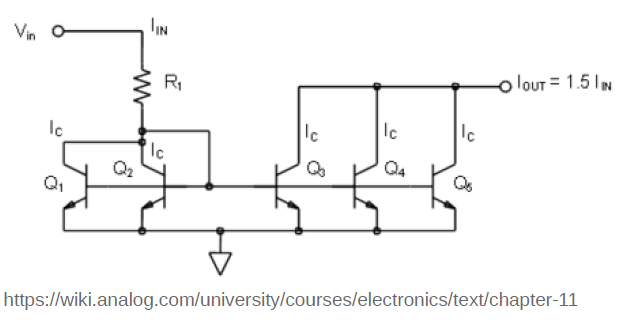
\includegraphics[width=10cm]{images/mirroir_courant_3.png}
\end{center}

Expliquez le fonctionnement et l'intérêt de ce montage.
}

On retrouve dans ce montage la même structure que dans le premier exercice : un miroir de courant.

La structure proposée a N transistors du côté pilotage (IN) et M transistors du côté puissance (OUT).

Tous les transistors sont identiques et ont pour relation : $I_{C} = \beta \cdot I_{B}$. On supposera $\beta >> 1$.

\textbf{Côté Pilotage (IN)}

Du côté pilotage ($V_{IN}$ et $I_{IN}$), on retrouve un nombre N de transistors (ici $N=2$).

D'après la formule obtenue dans l'exercice 1, on a un courant $$I_{IN} = N \cdot I_{C} + (N+M) \cdot I_{B}$$

En supposant $\beta >> 1$, on obtient alors que $I_{IN} = N \cdot I_C$.

\textbf{Côté Puissance (OUT)}

Du côté puissance ($I_{OUT}$), on retrouve un nombre M de transistors (ici $M=3$).

D'après la loi des noeuds : $I_{OUT} = M \cdot I_C$.

\textbf{Montage complet}

Le montage complet donne alors la relation suivante :

$$\boxed{I_{OUT} = \frac{M}{N} \cdot I_{IN}}$$

Dans le cas proposé, $N=2$ et $M=3$ donnent bien $I_{OUT} = 1.5 \cdot I_{IN}$.

Ce montage permet de modifier le rapport de courants entre l'entrée et la sortie, par une mise en parallèle des courants.

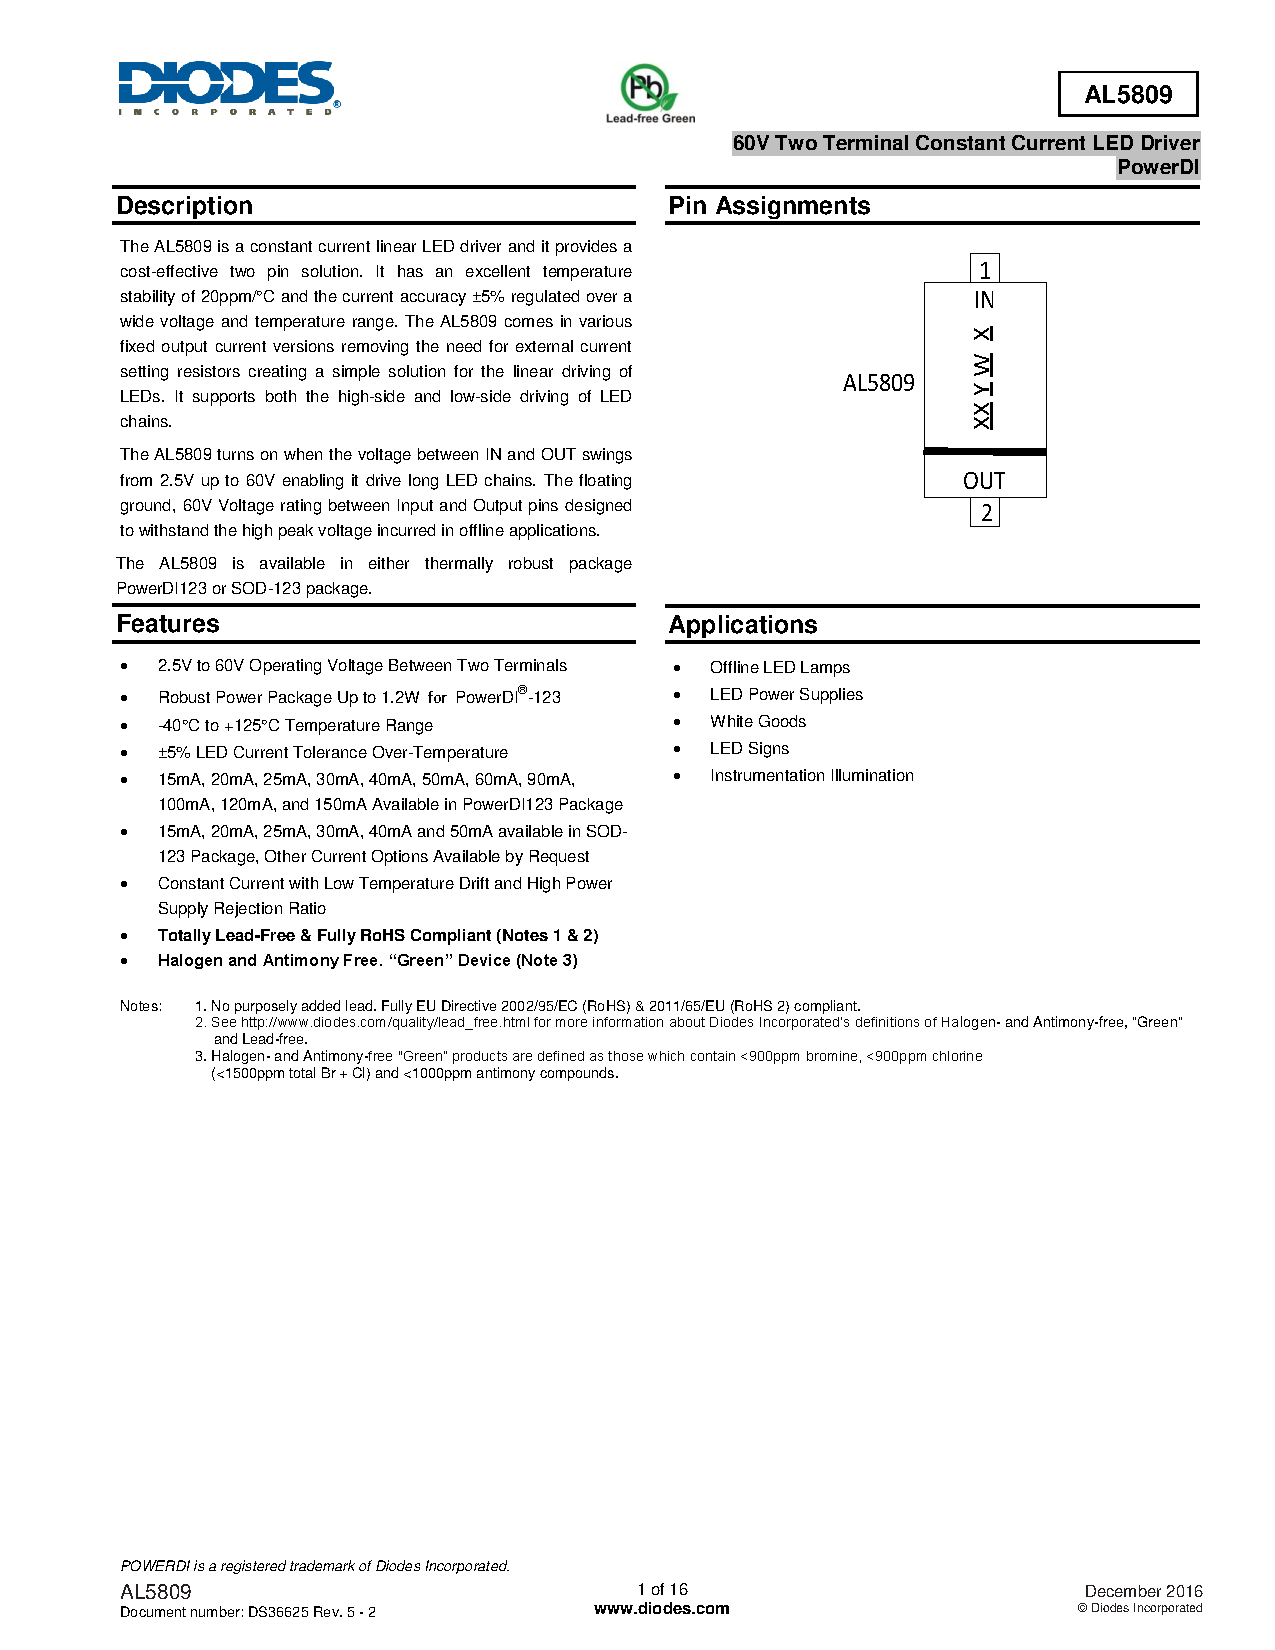
\includepdf[pages={1-2,4-5}]{docs/AL5809.pdf}

\end {document}